\documentclass[
  final,
  babelLanguage=british,
  desktopVersion,
  %showtrims,
  %overleaf,
]{anecdote}

%\graphicspath{{./assets/photos/300dpi/}}
\graphicspath{{./assets/photos/92dpi/}}

% NOTE: pdfinfo tags and hyperref metadata are set in the documentclass.

% Page size: 6x9 inch
% Body text: 10.5 / 15 pt

\usepackage{local}

%% Details of the book
%% ===================

\title{Prophecy Title}
\subtitle{Prophecy Subtitle}
\author{The Author}
\publisher{The Publisher}
\date{2017-08-19}
\editionInfo{\textit{First edition}, printed in TODO Country, 2017}% TODO update edition info
\ISBN{000-000-0000-00-0}% TODO update ISBN

% === Metadata ===

\pdfinfo{%
  /Title (\thetitle)%
  /Author (\theauthor)
  /Subject (subject)% TODO subject
  /Keywords (keywords)% TODO keywords
  /GTS_PDFXVersion (PDF/X-1:2001)%
  /GTS_PDFXConformance (PDF/X-1a:2001)%
}

%% === Load further packages ===

%% === Hyphenation exceptions and corrections ===

\hyphenation{London}

\begin{document}

\frontmatter

\ifdesktopversion
\desktopCover{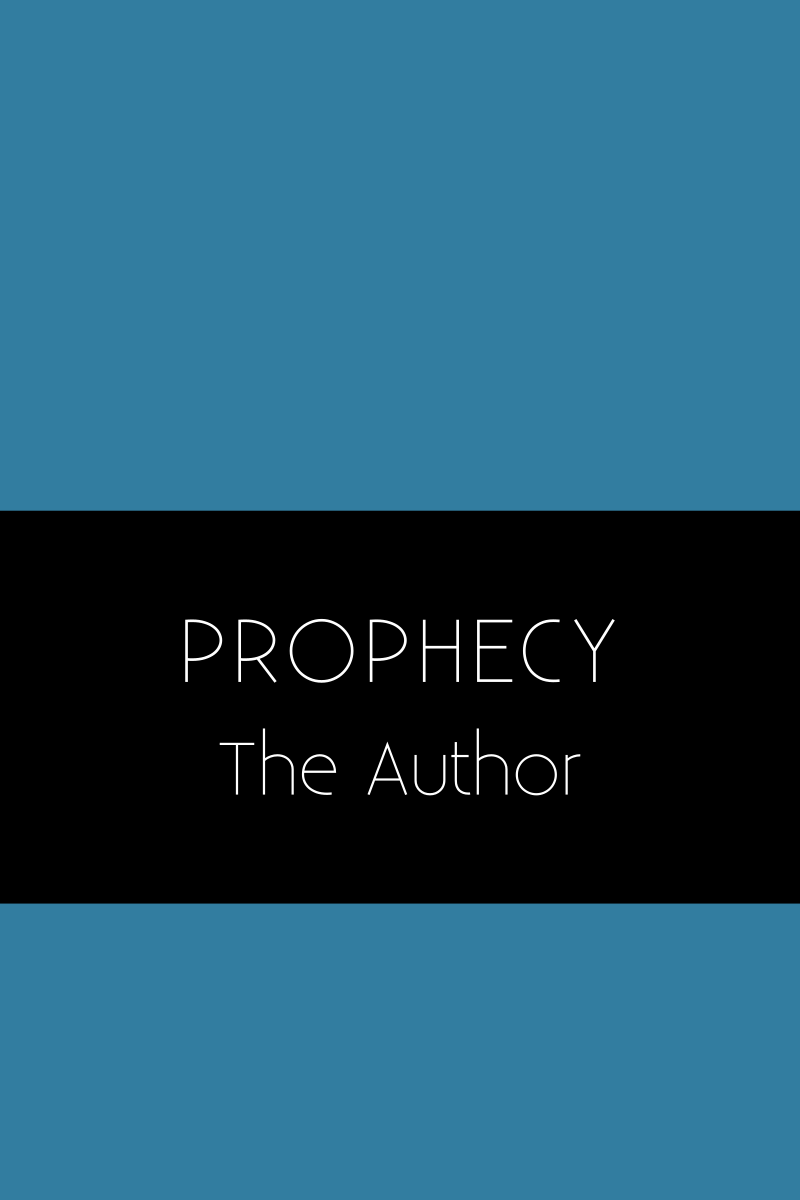
\includegraphics[height=\paperheight]{./desktop-cover.png}}
\fi

\cleartorecto
\thispagestyle{empty}
\vspace*{5em}

{\centering

\settowidth{\titleLength}{%
  {\Large\chapterTitleFont\scshape\MakeLowercase{\thetitle}}%
}

{\Large\chapterTitleFont\scshape\MakeLowercase{\thetitle}}\\[0.3\baselineskip]
\setlength{\xheight}{\heightof{X}}
\raisebox{0.5\xheight}{\color[gray]{0.4}\rule{\titleLength}{0.25pt}}\\[0.3\baselineskip]
{\itshape
\thesubtitle}

\vfill

\theauthor

\vspace*{5em}

}



\cleartoverso
\thispagestyle{empty}

{\copyrightsize
\centering
\setlength{\parindent}{0pt}%
\setlength{\parskip}{0.8\baselineskip}%

\thetitle\\
por \theauthor

Publicações Sumedhārāma\\
\href{http://sumedharama.pt}{www.sumedharama.pt}

As publicações de Sumedharama são para distribuição gratuita. Na maioria
dos casos, isto é possível graças a doações, de indivíduos ou grupos,
feitas especificamente para que as publicações dos ensinamentos do
Buddha possam estar disponíveis gratuitamente.

\textit{Sabbadānaṃ dhammadānaṃ jinati}\\
`A oferta de Dhamma é superior a qualquer outra oferta.'

Este livro encontra-se disponível para distribuição gratuita em\\
\href{http://fsbooks.org/}{www.fsbooks.org}

ISBN \theISBN

Copyright \copyright\ Publicações Sumedhārāma 2018

Traduzido por Bhikkhu Appamādo

Tradução autorizada da edição inglesa:

\emph{Mindfulness: The Path to the Deathless}\\
Published by Amaravati Publications, 1987

\vfill

{\footnotesize

Este trabalho está licenciado com uma Licença Creative Commons\\
Atribuição-NãoComercial-SemDerivações 4.0 Internacional.

Veja página \pageref{copyright-details} para mais detalhes sobre direitos e restrições desta licença.

Produzido com o sistema tipográfico \LaTeX.\\
Fonte utilizada: Gentium e Crimson~Roman.

\theEditionInfo

}}


\cleartorecto
\thispagestyle{empty}

\mbox{}\vfill

\begin{verse}

{\itshape
Lorem ipsum dolor sit amet,\\
consectetuer adipiscing elit.
}


\end{verse}

\vfill\mbox{}


\cleartorecto
\tableofcontents*

\chapter{Foreword}

Nullam eu ante vel est convallis dignissim. Fusce suscipit, wisi nec facilisis
facilisis, est dui fermentum leo, quis tempor ligula erat quis odio. Nunc porta
vulputate tellus. Nunc rutrum turpis sed pede. Sed bibendum. Aliquam posuere.
Nunc aliquet, augue nec adipiscing interdum, lacus tellus malesuada massa, quis
varius mi purus non odio. Pellentesque condimentum, magna ut suscipit hendrerit,
ipsum augue ornare nulla, non luctus diam neque sit amet urna. Curabitur
vulputate vestibulum lorem. Fusce sagittis, libero non molestie mollis, magna
orci ultrices dolor, at vulputate neque nulla lacinia eros. Sed id ligula quis
est convallis tempor. Curabitur lacinia pulvinar nibh. Nam a sapien.

\bigskip

{\raggedleft
  Reviewer Person\\
  July 2017
\par}


\chapter{Antes de começar}

A maior parte destas instruções podem ser levadas a cabo quer estejamos
sentados, em pé ou a andar. Contudo, estar consciente da respiração
(\emph{ānāpānasati}) tal como apresentado nos primeiros capítulos é algo
geralmente realizado na postura de sentado, uma vez que esse trabalho é
potenciado quando realizado num estado físico de quietude e
estabilidade. Para este estado a ênfase é sentarmo"-nos de forma a que a
coluna esteja erguida mas não em esforço, com o pescoço alinhado com a
coluna e a cabeça em equilíbrio de forma a não pender para a frente. É
de opinião geral que a postura de lótus de pernas cruzadas (sentados
numa almofada ou num tapete, com um ou ambos os pés colocados na coxa
oposta, com as plantas dos pés para cima) confere um equilíbrio ideal
entre esforço e estabilidade -- após alguns meses de prática. É bom
treinarmo"-nos gentilmente nesta direcção, um pouco de cada vez. Se esta
postura for muito difícil pode ser usada uma cadeira de costas direitas.

Após ter"-se alcançado estabilidade e um certo equilíbrio físico, a cara
e os braços devem ficar descontraidos, com as mãos a descansar no colo,
uma na palma da outra. Deixem as pálpebras fecharem"-se, relaxem a mente
\ldots{} escolham o objecto de meditação.

\emph{Jongrom}, uma palavra Tailandesa derivada do Pāli (linguagem das
escrituras) `\emph{caṅkama}' significa passear para a frente e para trás
num caminho a direito. O caminho deve ser medido, sendo o ideal vinte a
trinta passos entre dois objectos claramente
identificáveis de modo a não ter que contar os passos enquanto
pratica o \emph{jongrom}. As mãos deverão estar unidas de uma forma
suave, à frente ou atrás do corpo, com os braços relaxados. O olhar
deverá estar direccionado no caminho sem se focar nele, a uma distância
de aproximadamente dez passos à frente, não para observar nada em
particular mas para manter o ângulo mais confortável para o pescoço. O
caminhar começa então com uma postura correcta e quando se chega ao fim
do percurso devemos permanecer imóveis por um período que pode durar uma
ou duas respirações. Então, conscientemente, viramo"-nos e recomeçamos a
andar no sentido contrário.



% Page 1 is the first page of the first chapter.
\mainmatter

\chapterNote{Chapter one subtitle}

\chapter{Chapter One Title}
\tocChapterNote{Chapter one subtitle}

Aliquam erat volutpat. Nunc eleifend leo vitae magna. In id erat non orci
commodo lobortis. Proin neque massa, cursus ut, gravida ut, lobortis eget,
lacus. Sed diam. Praesent fermentum tempor tellus. Nullam tempus. Mauris ac
felis vel velit tristique imperdiet. Donec at pede. Etiam vel neque nec dui
dignissim bibendum. Vivamus id enim. Phasellus neque orci, porta a, aliquet
quis, semper a, massa. Phasellus purus. Pellentesque tristique imperdiet tortor.
Nam euismod tellus id erat.


\chapterNote{Chapter two subtitle}

\chapter{Chapter Two Title}
\tocChapterNote{Chapter two subtitle}

Nullam eu ante vel est convallis dignissim. Fusce suscipit, wisi nec facilisis
facilisis, est dui fermentum leo, quis tempor ligula erat quis odio. Nunc porta
vulputate tellus. Nunc rutrum turpis sed pede. Sed bibendum. Aliquam posuere.
Nunc aliquet, augue nec adipiscing interdum, lacus tellus malesuada massa, quis
varius mi purus non odio. Pellentesque condimentum, magna ut suscipit hendrerit,
ipsum augue ornare nulla, non luctus diam neque sit amet urna. Curabitur
vulputate vestibulum lorem. Fusce sagittis, libero non molestie mollis, magna
orci ultrices dolor, at vulputate neque nulla lacinia eros. Sed id ligula quis
est convallis tempor. Curabitur lacinia pulvinar nibh. Nam a sapien.




\backmatter

\chapter{Glossary}

\begin{glossarydescription}

% === A ===

\item[anicca] (Pali) Impermanence: one of the \emph{three characteristics of
    existence} along with not-self (\emph{anattā}) and unsatisfactoriness
  (\emph{dukkha}).

% === B ===

\item[borapet] (Thai) Tinospora crispa. Heart-shaped moonseed or guduchi.
  An extremely bitter vine used as a prophylactic and treatment for malaria.

% === C ===

% === D ===

% === E ===

% === F ===

% === G ===

% === H ===

% === I ===

% === J ===

% === K ===

% === L ===

% === M ===

% === N ===

% === O ===

% === P ===

% === Q ===

% === R ===

% === S ===

% === T ===

% === U ===

% === V ===

% === W ===

\end{glossarydescription}



\cleartorecto
\thispagestyle{plain}

{\fontsize{10}{14}\selectfont%
\setlength{\parindent}{0pt}%
\raggedright\label{copyright-details}%
\setlength{\parskip}{7pt}%

{\centering

{\LARGE\ccbyncnd}

This work is licensed under a Creative Commons\\
Attribution-NonCommercial-NoDerivatives 4.0 International~License.\footnote{%
\href{http://creativecommons.org/licenses/by-nc-nd/4.0/}{http://creativecommons.org/licenses/by-nc-nd/4.0/}}

}

You are free to:

\begin{packeditemize}
\item Share — copy and redistribute the material in any medium or format
\end{packeditemize}

The licensor cannot revoke these freedoms as long as you follow the license terms.

Under the following terms:

\begin{packeditemize}
\item Attribution — You must give appropriate credit, provide a link to the license, and indicate if changes were made. You may do so in any reasonable manner, but not in any way that suggests the licensor endorses you or your use.
\item NonCommercial — You may not use the material for commercial purposes.
\item NoDerivatives — If you remix, transform, or build upon the material, you may not distribute the modified material.
\end{packeditemize}

No additional restrictions — You may not apply legal terms or technological measures that legally restrict others from doing anything the license permits.

Notices:

You do not have to comply with the license for elements of the material in the public domain or where your use is permitted by an applicable exception or limitation.

No warranties are given. The license may not give you all of the permissions necessary for your intended use. For example, other rights such as publicity, privacy, or moral rights may limit how you use the material.

% TODO confirm this notice with The Publisher

\thePublisher\ asserts its moral right to be identified as the author of this book.

\thePublisher\ requests that you attribute ownership of the work to \thePublisher\ on copying, distribution, display or performance of the work.

}

% Add an extra page to complete the last sheet.
\ifodd\thepage
\newpage\thispagestyle{empty}\mbox{}
\fi

\end{document}
